\chapter{Nestor1: dredging and dumping}








%\newpage
%****************************************************
\section{General information about usage of Nestor } \label{sec:E1GenInfo}
%****************************************************
%
%x\textcolor{white}{force a empty line by white lettering}\\ %----- white line-----
%x\\
%****************************************************
\subsection{Nestor in the steering files} \label{ssec:E1SteerF}
%
%x\textcolor{white}{force a empty line by white lettering}\\ %----- white line-----
%x\\
%x\\
\fcolorbox{green}{yellow}{
  \parbox{1.0\linewidth}{Nestor settings in the \textsc{Gaia/Telemac2d Steering File}:\\
  \\ \hspace*{3mm} \texttt{\small{NESTOR~~~~~~~~~~~~~~~~~~~~~~~~=~YES}}
  \\ \hspace*{3mm} \texttt{\small{NESTOR~ACTION~FILE~~~~~~~~~~~~=~name of the Action file}}
  \\ \hspace*{3mm} \texttt{\small{NESTOR~POLYGON~FILE~~~~~~~~~~~=~name of the polygon file}}
  \\ \hspace*{3mm} \texttt{\small{NESTOR~SURFACE~REFERENCE~FILE~=~name of the reference level file}}
  \\ \hspace*{3mm} \texttt{\small{NESTOR~RESTART~FILE~~~~~~~~~~~=~optional}}
  \\ \hspace*{3mm} \texttt{\small{ORIGINAL~DATE~OF~TIME~~~~~~~~~=~2000;01;01}}
  \\ \hspace*{3mm} \texttt{\small{ORIGINAL~HOUR~OF~TIME~~~~~~~~~=~0;0;0}}
}}
\textcolor{white}{force a empty line by white lettering}\\ %----- white line-----
Because the reference level file contains the flow length coordinates which are attached to the sections (fig.\,\ref{E3grid}),
the reference level file must exist, even if it is not adressed by an Action.
The file must contain at least two sections which define an area that covers all polygons (fig.\,\ref{refl3D},\,\ref{geom2D}).
The flow length coordinates are required to print the NodeInfo line (chpt.\,\ref{sssec:E1NodeInfo}\,/\,page\,\pageref{txt:E1XdigX})
%x\\
%x\\
%****************************************************
\subsection{General structure of the \textsc{Nestor Action File}} \label{ssec:E1GenActF}
%
\fcolorbox{green}{yellow}{
  \parbox{1.0\linewidth}{General structure of the \textsc{Nestor Action File} ( = steering file for Nestor):\\
  \\ \hspace*{3mm} \texttt{\small{RESTART~=~FALSE/TRUE}}
  \\ \hspace*{3mm} \texttt{\small{/ \textit{comment line}}}
  \\ \hspace*{3mm} \texttt{\small{ACTION}}
  \\ \hspace*{3mm} \texttt{\small{~~ActionType~=~...}}
  \\ \hspace*{3mm} \texttt{\small{~~~~~~...}}
  \\ \hspace*{3mm} \texttt{\small{ENDACTION}}
  \\ \hspace*{3mm} \texttt{\small{...}}
  \\ \hspace*{3mm} \texttt{\small{ACTION}}
  \\ \hspace*{3mm} \texttt{\small{~~ActionType~=~...~~~~/ \textit{comment at the end of a line}}}
  \\ \hspace*{3mm} \texttt{\small{~~~~~~...}}
  \\ \hspace*{3mm} \texttt{\small{ENDACTION}}
  \\ \hspace*{3mm} \texttt{\small{ENDFILE}}\\
  \\Inside the block \texttt{\small{~ACTION - ENDACTION~}} all other keywords,
    excluding \texttt{GrainClass} (chpt.\,\ref{ssec:E1SuppMat}\,/\,page \pageref{txt:SupplyMaterial}), may appear in any order.
}}





%\newpage
%****************************************************
\subsection{About Nestor polygons}  \label{ssec:E1Poly}
%
\textcolor{white}{force a empty line by white lettering}\\ %----- white line-----
%x\\
%x\\
\fcolorbox{green}{yellow}{
  \parbox{1.0\linewidth}{General structure of the \textsc{Nestor Polygon File}:\\
  \\ \hspace*{3mm} \texttt{\small{/\textit{this is a comment line}}}
  \\ \hspace*{3mm} \texttt{\small{\#\textit{this is a comment line as well}}}
  \\ \hspace*{3mm} \texttt{\small{NAME:polygon\_name~~~~}}
  \\ \hspace*{3mm} \texttt{\small{~~~x-koord~~~~y-koord}}
  \\ \hspace*{3mm} \texttt{\small{~~~x-koord~~~~y-koord}}
  \\ \hspace*{3mm} \texttt{\small{~~~:~~~~~~~~~~:~~~~~~}}
  \\ \hspace*{3mm} \texttt{\small{NAME:polygon\_name~~~}}
  \\ \hspace*{3mm} \texttt{\small{~~~x-koord~~~~y-koord}}
  \\ \hspace*{3mm} \texttt{\small{~~~x-koord~~~~y-koord}}
  \\ \hspace*{3mm} \texttt{\small{~~~:~~~~~~~~~~:~~~~~~}}
  \\ \hspace*{3mm} \texttt{\small{ENDFILE}}\\
  \\
  The keyword \texttt{~NAME:~} induces a new polygon.\\
  The polygon name must start right after the colon.\\
}}
\textcolor{white}{force a empty line by white lettering} \\    %----- white line-----
%x\\
\fcolorbox{green}{yellow}{
  \parbox{1.0\linewidth}{Convention regarding to polygons:
  \begin{itemize}
     \item{The polygon name must start with an unique integer number between 100 and 999.
           Any text after that is treated as a comment to help the user.\\
           Example:\texttt{~123anyString}}\\
           Internally only the number is used to identify the polygon.
     \item{Multiple assignements are not allowed. That means a polygon may be assigned
           only to one Action. (The assignements are defined in the Action file.)}
  \end{itemize}
}}
\textcolor{white}{force a empty line by white lettering} \\    %----- white line-----
\\

%****************************************************
\subsection{About supply material}  \label{ssec:E1SuppMat}
%
\textcolor{white}{force a empty line by white lettering}\\ %----- white line-----
\label{txt:SupplyMaterial}
\fcolorbox{green}{yellow}{
  \parbox{1.0\linewidth}{Convention for definition of the supply material:
  \begin{itemize}
  \item{The sum of the fractions of the grain classes must be 1.}
  \item{The number of the grain classes must be the same as set in the \textsc{Gaia Steering File}.}
  \item{The order of the grain classes must appear in the Action block in the same order as
        they are set in the \textsc{Gaia Steering File}.}
  \end{itemize}
}}
%x\\
%x\\






%%****************************************************
%\subsection{About dumping (after dredging)}
%%
%\textcolor{white}{force a empty line by white lettering} \\    %----- white line-----
%\\
%\\
%\fcolorbox{green}{yellow}{
%  \parbox{1.0\linewidth}{Convention for dumping in case of \texttt{~Dig\_by\_time~} or \texttt{~Dig\_by\_criterion~}:
%  \begin{itemize}
%  \item{\texttt{FieldDump~} is optional. Only when a polygon name is assigned to the keyword
%        will the dredged material be dumped, otherwise dumping won't happen.}
%  \item{With \texttt{~Dig\_by\_time~} the keyword \texttt{~DumpRate~} is optional.
%        In case it is not used, dumping and dredging finalises at the same time (\texttt{~TimeEnd~}).}
%  \end{itemize}
%}}




\newpage
%****************************************************
\subsection{Information about Nestor in the Telemac listing file} \label{ssec:E1ListiF}
%
\textcolor{white}{force a empty line by white lettering}\\ %----- white line-----
\fcolorbox{green}{yellow}{
  \parbox{1.0\linewidth}{In order to find specific Nestor information in the Telemac listing file about:
    \begin{itemize}
    \item{which Action was when active and what was going on, search for \texttt{~"\textbf{?>}"~} (see below or chpt.\,\ref{sec:E1Result}\,/\,page\,\pageref{txt:E1List})}
    \item{what was the users mistake, search for \texttt{~"\textbf{?> error}"~} (see below)}
    \item{the dredged volume, search for \texttt{~"\textbf{XdigX}"~} (see chpt.\,\ref{sssec:E1NodeInfo})}
    \item{the dumped volume, search for \texttt{~"\textbf{XdumX}"~}}
    \end{itemize}
    \textbf{In case of parallel computation you have to search in the listing file of each partition ! }
 }}
\textcolor{white}{force a empty line by white lettering}\\ %----- white line-----
Excerpt from the telemac listing with information about the Action status:
  \\ \hspace*{3mm} \texttt{\small{~?>~:}}
  \\ \hspace*{3mm} \texttt{\small{~?>~info:========================================================+}}
  \\ \hspace*{3mm} \texttt{\small{~?>~info:~~~~~~~~~~~~NESTOR~~~~~~~~~~~~~~~~~~~~~~~~~~~~~~~~~~~~~~|}}
  \\ \hspace*{3mm} \texttt{\small{~?>~~~~~~~~~~~~~~~~~~~~~~~~~~~~~~~~~~~~~~~~~~~~~~~~~~~~~~~~~~~~~~~}}
  \\ \hspace*{3mm} \texttt{\small{~?>~~~~~~~~~~action~number~~~~:~~~1~~~~~~~~~~~~~~~~~~~~~~~~~~~~~~~}}
  \\ \hspace*{3mm} \texttt{\small{~?>~~~~~~~~~~~~~~~~~~~~~~~~~~~~~~~~~~~~~~~~~~~~~~~~~~~~~~~~~~~~~~~}}
  \\ \hspace*{3mm} \texttt{\small{~?>~~~~~~~~~~start~action~~~~~:~Dig\_by\_time~~~~~~~~~~~~~~~~~~~~~~~}}
  \\ \hspace*{3mm} \texttt{\small{~?>~~nominal~start~time~~[s]~~:~~~~50.000000000000000~~~~~~~~~~~~~}}
  \\ \hspace*{3mm} \texttt{\small{~?>~~~~~~~~~~start~time~~[s]~~:~~~~50.000000000000000~~~~~~~~~~~~~}}
  \\ \hspace*{3mm} \texttt{\small{~?>~~~~~~~~~~~~~~~~~~~~~~~~~~~~~~~~~~~~~~~~~~~~~~~~~~~~~~~~~~~~~~~}}
  \\ \hspace*{3mm} \texttt{\small{~?>~~~~~~~~~~FieldDig~~~~~~~~~:~201\_Abschnitt\_1\_2\_1000m**2~~~~~~~~}}
  \\ \hspace*{3mm} \texttt{\small{~?>~~~~~dz~per~time~step~[m]~~:~~~1.00000000000000002E-003~~~~~~~~}}
  \\ \hspace*{3mm} \texttt{\small{~?>~~~~~~~~~~~~~~~~~~~~~~~~~~~~~~~~~~~~~~~~~~~~~~~~~~~~~~~~~~~~~~~}}
  \\ \hspace*{3mm} \texttt{\small{~?>~~~~~~~~~~FieldDump~~~~~~~~:~202\_Abschnitt\_6\_7\_1000m**2~~~~~~~~}}
  \\ \hspace*{3mm} \texttt{\small{~?>~~~~~dz~per~time~step~[m]~~:~~~5.00000000000000010E-004~~~~~~~~}}
  \\ \hspace*{3mm} \texttt{\small{~?>~~~~~~~~~~~~~~~~~~~~~~~~~~~~~~~~~~~~~~~~~~~~~~~~~~~~~~~~~~~~~~~}}
  \\ \hspace*{3mm} \texttt{\small{~?>~info:========================================================+}}
  \\ \hspace*{3mm} \texttt{\small{~?>~:}}\\
\\Excerpt from the Telemac listing file with information due to a user mistake:
  \\ \hspace*{3mm} \texttt{\small{?>~:}}
  \\ \hspace*{3mm} \texttt{\small{?>~error:========================================================+}}
  \\ \hspace*{3mm} \texttt{\small{?>~error:~~~~~~~~~~~error~in~dredge~module~Nestor~~~~~~~~~~~~~~~~|}}
  \\ \hspace*{3mm} \texttt{\small{?>~error:~~~~~~~~~~~~~~~~~~~~~~~~~~~~~~~~~~~~~~~~~~~~~~~~~~~~~~~~|}}
  \\ \hspace*{3mm} \texttt{\small{?>~error:~~occured~in~Subroutine~~~~~~~ReadDigActions}}
  \\ \hspace*{3mm} \texttt{\small{?>~error:~~occured~in~parallel~thread~~0}}
  \\ \hspace*{3mm} \texttt{\small{?>~error:}}
  \\ \hspace*{3mm} \texttt{\small{?>~error:~~while~read~the~Action~file}}
  \\ \hspace*{3mm} \texttt{\small{?>~error:~~reason:~~unknown~keyword:~~~~~xReferenceLevel}}
  \\ \hspace*{3mm} \texttt{\small{?>~error:~~~~~~~~~~~check~spelling~!}}
  \\ \hspace*{3mm} \texttt{\small{?>~error:~~occured~in~line:~~~~~10}}
  \\ \hspace*{3mm} \texttt{\small{?>~error:~~~~~~~~~~~~~~~~~~~~~~~~~~~~~~~~~~~~~~~~~~~~~~~~~~~~~~~~|}}
  \\ \hspace*{3mm} \texttt{\small{?>~error:========================================================+}}
  \\ \hspace*{3mm} \texttt{\small{?>~:}}
%
%
\newpage
\setcounter{secnumdepth}{3}
\subsubsection{Node Information} \label{sssec:E1NodeInfo} \label{txt:E1XdigX}
While a Nestor Action is active, the elevation of the nodes inside the assigned polygon (working area)
will be changed every time step a little bit.
At the time step, when an Action changes a node the last time, a "NodeInfo" line will be printed in the Telemac listing file.
Each info line is marked with the lable \texttt{~"\textbf{XdigX}"~} or \texttt{~"\textbf{XdumX}"~} at the beginning and followed by the values shown below
\begin{itemize}
   \item{\texttt{TimeStart~~~~~}\textit{of the Action-X \qquad[s]$^{(*)}$}}
   \item{\texttt{Time~~~~~~~~~~}\textit{when the last change to the node happened \qquad[s]$^{(*)}$ }}
   \item{\texttt{Delta-Z~~~~~~~}\textit{total evolution caused by Action-X \qquad[m]}}
   \item{\texttt{Delta-Volume~~}\textit{= Delta-Z * node area \qquad[m$^3$]}}
   \item{\texttt{Index~~~~~~~~~}\textit{global number of node}}
   \item{\texttt{Km~~~~~~~~~~~~}\textit{flow length coordinate \qquad[km]}}
   \item{\texttt{X-coordinate~~}\textit{[m]}}
   \item{\texttt{Y-coordinate~~}\textit{[m]}}
   \item{\texttt{Name~~~~~~~~~~}\textit{of the assigned polygon}}
   \item{\texttt{Action~~~~~~~~}\textit{number of the Action}}
\end{itemize}
$^{(*)}$ \small{seconds since simulation start}\\
\\
Excerpt of listing file with NodeInfo lines :
\\ \hspace*{3mm} \texttt{\scriptsize{~:}}
\\ \hspace*{3mm} \texttt{\scriptsize{XdigX~800.00~820.00~~10.73~~10.12~~~853~~~1.871~~1058.3149~~-708.833~~~100\_Fairway~~1}}
\\ \hspace*{3mm} \texttt{\scriptsize{XdigX~800.00~824.00~~14.89~~15.44~~1502~~~1.175~~1167.8081~~-153.119~~~100\_Fairway~~1}}
\\ \hspace*{3mm} \texttt{\scriptsize{XdumX~900.00~960.00~~14.95~~13.96~~1042~~~2.797~~949.61357~~~1302.40~~~100\_Fairway~~2}}
\\ \hspace*{3mm} \texttt{\scriptsize{~:}}\\
\\
\newpage
%****************************************************
\subsection{Tables of Nestor keywords} \label{ssec:E1KeyTabl}
%
\begin{table}[ht]
\centering
\caption{ Keywords for Nestor Action \texttt{~Dig\_by\_time~}}
\begin{tabular}{| l | l | l | l | p{4.7cm} |}
\hline
{\textcolor{white}{\LARGE |}} \textbf{KEYWORD}        &     &\textbf{VALUE}         &\textbf{UNIT}          &\textbf{COMMENT}     \\ \hline
{\textcolor{white}{\LARGE |}} \texttt{ActionType}     &     &\texttt{Dig\_by\_time} &                       &                     \\ \hline
{\textcolor{white}{\LARGE |}} \texttt{TimeStart}      &     &date-time              &\multicolumn{2}{l|}{[ $yyyy.mm.dd-hh:mm:ss$ ]} \\ \hline
{\textcolor{white}{\LARGE |}} \texttt{TimeEnd}        &     &date-time              &\multicolumn{2}{l|}{[ $yyyy.mm.dd-hh:mm:ss$ ]} \\ \hline
{\textcolor{white}{\LARGE |}} \texttt{FieldDig}       &     &polygon name           &                       &                     \\ \hline
{\textcolor{white}{\LARGE |}} \texttt{DigVolume}      &     &real                   &[ $m^3$ ]              &                     \\ \hline
{\textcolor{white}{\LARGE |}} \texttt{FieldDump}      &opt. &polygon name           &                       &dumping happens only if set \\ \hline
{\textcolor{white}{\LARGE |}} \texttt{DumpRate}       &opt. &real                   &[ $m/s$ ]                &if not set, dumping ends at TimeEnd \\ \hline
{\textcolor{white}{\LARGE |}} \texttt{DumpPlanar}     &opt. &\texttt{FALSE} (\small{default}) &             &                     \\
{\textcolor{white}{\LARGE |}}                         &     &\texttt{TRUE}                    &             &                     \\ \hline
{\textcolor{white}{\LARGE |}} \texttt{ReferenceLevel} &opt. &\texttt{GRID}          &                       &must be set if       \\
{\textcolor{white}{\LARGE |}}                         &     &\texttt{SECTIONS}      &                       &DumpPlanar = TRUE    \\
{\textcolor{white}{\LARGE |}}                         &     &\texttt{WATERLVL1}     &                       &                     \\
{\textcolor{white}{\LARGE |}}                         &     &\texttt{WATERLVL2}     &                       &                     \\
{\textcolor{white}{\LARGE |}}                         &     &\texttt{WATERLVL3}     &                       &                     \\ \hline
\multicolumn{5}{|l|}{{\textcolor{white}{\LARGE |}}\small{opt.: optional}}                                                        \\ \hline
\end{tabular}
\end{table}


\begin{table}[ht]
\centering
\caption{Keywords for Nestor Action \texttt{~Dump\_by\_time~}}
\begin{tabular}{| l | l | l | l | p{4.5cm} |}
\hline
{\textcolor{white}{\LARGE |}} \textbf{KEYWORD}        &     &\textbf{VALUE}         &\textbf{UNIT}          &\textbf{COMMENT}     \\ \hline
{\textcolor{white}{\LARGE |}} \texttt{ActionType}     &     &\texttt{Dump\_by\_time}&                       &                     \\ \hline
{\textcolor{white}{\LARGE |}} \texttt{TimeStart}      &     &date-time              &\multicolumn{2}{l|}{[ $yyyy.mm.dd-hh:mm:ss$ ]} \\ \hline
{\textcolor{white}{\LARGE |}} \texttt{TimeEnd}        &     &date-time              &\multicolumn{2}{l|}{[ $yyyy.mm.dd-hh:mm:ss$ ]} \\ \hline
{\textcolor{white}{\LARGE |}} \texttt{FieldDump}      &     &polygon name           &                       &                     \\ \hline
{\textcolor{white}{\LARGE |}} \texttt{DumpVolume}     &     &real                   &[ $m^3$ ]              &                     \\ \hline
{\textcolor{white}{\LARGE |}} \texttt{GrainClass}     &     &real                   &                       &the sum of all grain \\
{\textcolor{white}{\LARGE |}} \texttt{:}              &     &real                   &                       &classes must be 1.0  \\
{\textcolor{white}{\LARGE |}} \texttt{GrainClass}     &     &real                   &                       &see\,chpt.\,\ref{ssec:E1SuppMat}\\ \hline
{\textcolor{white}{\LARGE |}} \texttt{DumpPlanar}     &opt. &\texttt{FALSE} (\small{default}) &             &                     \\
{\textcolor{white}{\LARGE |}}                         &     &\texttt{TRUE}                    &             &                     \\ \hline
{\textcolor{white}{\LARGE |}} \texttt{ReferenceLevel} &opt. &\texttt{GRID}          &                       &must be set if       \\
{\textcolor{white}{\LARGE |}}                         &     &\texttt{SECTIONS}      &                       &DumpPlanar = TRUE    \\
{\textcolor{white}{\LARGE |}}                         &     &\texttt{WATERLVL1}     &                       &                     \\
{\textcolor{white}{\LARGE |}}                         &     &\texttt{WATERLVL2}     &                       &                     \\
{\textcolor{white}{\LARGE |}}                         &     &\texttt{WATERLVL3}     &                       &                     \\ \hline
\multicolumn{5}{|l|}{{\textcolor{white}{\LARGE |}}\small{opt.: optional}}                                                        \\ \hline
\end{tabular}
\end{table}


\begin{table}[ht]
\centering
\caption{Keywords for Nestor Action \texttt{~Dig\_by\_criterion~}}
\begin{tabular}{| l | l | l | l | p{2.6cm} |}
\hline
{\textcolor{white}{\LARGE |}} \textbf{KEYWORD}        &     &\textbf{VALUE}         &\textbf{UNIT}          &\textbf{COMMENT}     \\ \hline
{\textcolor{white}{\LARGE |}} \texttt{ActionType}     &     &\texttt{Dig\_by\_criterion}&                   &                     \\ \hline
{\textcolor{white}{\LARGE |}} \texttt{TimeStart}      &     &date-time              &\multicolumn{2}{l|}{[ $yyyy.mm.dd-hh:mm:ss$ ]} \\ \hline
{\textcolor{white}{\LARGE |}} \texttt{TimeRepeat}     &     &real                   &[ $s$ ]                &                     \\ \hline
{\textcolor{white}{\LARGE |}} \texttt{TimeEnd}        &     &date-time              &\multicolumn{2}{l|}{[ $yyyy.mm.dd-hh:mm:ss$ ]} \\ \hline
{\textcolor{white}{\LARGE |}} \texttt{FieldDig}       &     &polygon name           &                       &                     \\ \hline
{\textcolor{white}{\LARGE |}} \texttt{DigRate}        &     &real                   &[ $m/s$ ]              &                     \\ \hline
{\textcolor{white}{\LARGE |}} \texttt{CritDepth}      &     &real                   &[ $m$ ]                &                     \\ \hline
{\textcolor{white}{\LARGE |}} \texttt{DigDepth}       &     &real                   &[ $m$ ]                &                     \\ \hline
{\textcolor{white}{\LARGE |}} \texttt{MinVolume}      &     &real                   &[ $m^3$ ]              &                     \\ \hline
{\textcolor{white}{\LARGE |}} \texttt{MinVolumeRadius}&     &real                   &[ $m$ ]                &                     \\ \hline
{\textcolor{white}{\LARGE |}} \texttt{ReferenceLevel} &     &\texttt{GRID}          &                       &                     \\
{\textcolor{white}{\LARGE |}}                         &     &\texttt{SECTIONS}      &                       &                     \\
{\textcolor{white}{\LARGE |}}                         &     &\texttt{WATERLVL1}     &                       &                     \\
{\textcolor{white}{\LARGE |}}                         &     &\texttt{WATERLVL2}     &                       &                     \\
{\textcolor{white}{\LARGE |}}                         &     &\texttt{WATERLVL3}     &                       &                     \\ \hline
{\textcolor{white}{\LARGE |}} \texttt{FieldDump}      &opt. &polygon name           &                       &dumping happens only if set \\ \hline
{\textcolor{white}{\LARGE |}} \texttt{DumpRate}       &opt. &real                   &[ $m/s$ ]              &must be set if dumping\\ \hline
{\textcolor{white}{\LARGE |}} \texttt{DumpPlanar}     &opt. &\texttt{FALSE} (\small{default}) &             &                     \\
{\textcolor{white}{\LARGE |}}                         &     &\texttt{TRUE}                    &             &                     \\ \hline
\multicolumn{5}{|l|}{{\textcolor{white}{\LARGE |}}\small{opt.: optional}}                                                        \\ \hline
\end{tabular}
\end{table}


\newpage
\begin{table}[ht]
\centering
\caption{Keywords for Nestor Action \texttt{~Save\_water\_level~}}
\begin{tabular}{| l | l | l | l | p{4.4cm} |}
\hline
{\textcolor{white}{\LARGE |}}\textbf{KEYWORD}        &     &\textbf{VALUE}         &\textbf{UNIT}          &\textbf{COMMENT}     \\ \hline
{\textcolor{white}{\LARGE |}}\texttt{ActionType}     &     &\texttt{Save\_water\_level}&                   &                     \\ \hline
{\textcolor{white}{\LARGE |}}\texttt{TimeStart}      &     &date-time              &\multicolumn{2}{l|}{[ $yyyy.mm.dd-hh:mm:ss$ ]} \\ \hline
{\textcolor{white}{\LARGE |}}\texttt{ReferenceLevel} &     &\texttt{WATERLVL1}     &                       &                     \\
{\textcolor{white}{\LARGE |}}                        &     &\texttt{WATERLVL2}     &                       &                     \\
{\textcolor{white}{\LARGE |}}                        &     &\texttt{WATERLVL3}     &                       &                     \\ \hline
\end{tabular}
\end{table}


%\newpage
\begin{table}[h]
\centering
\caption{Keywords for Nestor Action \texttt{~Backfill\_to\_level~}}
\begin{tabular}{| l | l | l | l | p{3.5cm} |}
\hline
{\textcolor{white}{\LARGE |}} \textbf{KEYWORD}        &     &\textbf{VALUE}         &\textbf{UNIT}          &\textbf{COMMENT}     \\ \hline
{\textcolor{white}{\LARGE |}} \texttt{ActionType}     &     &\texttt{Backfill\_to\_level}&                  &                     \\ \hline
{\textcolor{white}{\LARGE |}} \texttt{TimeStart}      &     &date-time              &\multicolumn{2}{l|}{[ $yyyy.mm.dd-hh:mm:ss$ ]} \\ \hline
{\textcolor{white}{\LARGE |}} \texttt{TimeEnd}        &     &date-time              &\multicolumn{2}{l|}{[ $yyyy.mm.dd-hh:mm:ss$ ]} \\ \hline
{\textcolor{white}{\LARGE |}} \texttt{FieldDump}      &     &polygon name           &                       &                     \\ \hline
{\textcolor{white}{\LARGE |}} \texttt{CritDepth}      &     &real                   &[ $m$ ]                &                     \\ \hline
{\textcolor{white}{\LARGE |}} \texttt{ReferenceLevel} &     &\texttt{GRID}          &                       &                     \\
{\textcolor{white}{\LARGE |}}                         &     &\texttt{SECTIONS}      &                       &                     \\
{\textcolor{white}{\LARGE |}}                         &     &\texttt{WATERLVL1}     &                       &                     \\
{\textcolor{white}{\LARGE |}}                         &     &\texttt{WATERLVL2}     &                       &                     \\
{\textcolor{white}{\LARGE |}}                         &     &\texttt{WATERLVL3}     &                       &                     \\ \hline
{\textcolor{white}{\LARGE |}} \texttt{GrainClass}     &     &real                   &                       &the sum of all grain \\
{\textcolor{white}{\LARGE |}} \texttt{:}              &     &real                   &                       &classes must be 1.0  \\
{\textcolor{white}{\LARGE |}} \texttt{GrainClass}     &     &real                   &                       &see\,chpt.\,\ref{ssec:E1SuppMat}\\ \hline
{\textcolor{white}{\LARGE |}} \texttt{DumpRate}       &opt. &real                   &[ $m/s$ ]              &if not set, backfilling ends at TimeEnd\\ \hline
\multicolumn{5}{|l|}{{\textcolor{white}{\LARGE |}}\small{opt.: optional}}                                                        \\ \hline
\end{tabular}
\end{table}

\clearpage

\newpage
%
%****************************************************
% - Purpose & Problem description:
%     These first two parts give reader short details about the test case,
%     the physical phenomena involved and specify how the numerical solution will be validated
\section{Purpose (Dig\_by\_time)}
%****************************************************
%
Example for Nestor:\\
dredging and dumping of the dredged material\\
\\
Details about:
\begin{itemize}
\item{\texttt{ActionType = Dig\_by\_time}}
%\item{General structure of the \textsc{Nestor Polygon File~}}
%\item{Convention for the naming of polygons}
%\item{\texttt{FieldDump}}
\end{itemize}




%\newpage
%****************************************************
\section{Description of the problem}
%****************************************************
%
This example covers a test case for the dredging and dumping of recently dredged material.
Hydro- and morphodynamic processes are not looked at closely.\\
\\
Excerpt from the Action file \texttt{\_DigActions.dat} where the Action is defined:\\
\hspace*{3mm} \texttt{\small{/================================================================}}\\
\hspace*{3mm} \texttt{\small{ACTION}}                                                           \\
\hspace*{3mm} \texttt{\small{~~ActionType~~~~=~~Dig\_by\_time}}                                 \\
\hspace*{3mm} \texttt{\small{~~TimeStart~~~~~=~2000.01.01-00:00:50~~~~~/~[yyyy.mm.dd-hh:mm:ss]}}\\
\hspace*{3mm} \texttt{\small{~~TimeEnd~~~~~~~=~2000.01.01-00:02:30~~~~~/~[yyyy.mm.dd-hh:mm:ss]}}\\
\hspace*{3mm} \texttt{\small{~~FieldDig~~~~~~=~~201\_Abschnitt\_1\_2\_1000m**2}}                \\
\hspace*{3mm} \texttt{\small{~~DigVolume~~~~~=~~100.00~~~~~~~~~~~~~~~~~/~[~m**3~]}}             \\
                                                                                                \\
\hspace*{3mm} \texttt{\small{~~FieldDump~~~~~=~202\_Abschnitt\_6\_7\_1000m**2}}                 \\
\hspace*{3mm} \texttt{\small{~~DumpRate~~~~~~=~~0.0005~~~~~~~~~~~~~~~~~/~[~m/s~]}}              \\
\hspace*{3mm} \texttt{\small{~~DumpPlanar~~~~=~~FALSE}}                                         \\
\hspace*{3mm} \texttt{\small{ENDACTION}}                                                        \\
\hspace*{3mm} \texttt{\small{/================================================================}}\\
\\
\\
100\,m$^3$ material will be dredged in the polygon named \texttt{201\_Abschnitt\_1\_2\_1000m**2} over a time period of 100\,s.
The polygons are defined (chpt.\,\ref{ssec:E1Poly}) in the file \texttt{\_DigPolys.dat}.\\
This dredging field is located between meter 100.5 and meter 300.5 of a flume. The area of the field is 200 x 5
= 1000\,m$^2$. In this part of the flume only coarse material (d\,=\,2\,mm) is present (fig.~\ref{E1iniDm}).
The date when the simulation starts is set in the GAIA steering file
\texttt{~gai\_nestor1.cas~} through the keywords:\\
\texttt{ORIGINAL DATE OF TIME = 2000;01;01}\\
\texttt{ORIGINAL HOUR OF TIME = 0;0;0}\\
The total simulation period of 250\,s is computed in 1\,s time steps.
The simulation starts at 2000.01.01-00:00:00 and 50\,s later, at 2000.01.01-00:00:50, the dredging starts.
Dredging then ends 100\,s later at 2000.01.01-00:02:30.
This is defined in the \textsc{Nestor Action File}.

Due to the dredging the bottom is lowered about 0,1\,m in the dredging area.
The dredging rate (calculated by Nestor) is the dredging volume devided by the dredging time and the dredging area
$\frac{100 m^3/s}{100 s*1000 m^2}=0.001$\,m/s

At the time when dredging starts the dredged material will
be dumped in the polygon named \texttt{~202\_Abschnitt\_6\_7\_1000m**2}, which is located between meter 700.5 and 900.5 of the flume.
The area of the dump field is 200 x 5 = 1000\,m$^2$.
At the start of the simulation, only fine material (d\,=\,0.1\,mm) is located here.
Due to the dumping rate (preset to 0.0005\,m/s), which is half the dredging rate, it takes 200\,s to dump the material.
In the end a 0.1\,m thick layer of dredged material will be deposited in the dumping field.

The sediment distribution will not be changed in the dredging area but in the dumping area.
There the mean grain size will be increased during the dumping of coarse material.
In the dumping area the final mean grain size is about 1.3\,mm (fig.\,\ref{E1endDm}) due to mixing processes of the Hirano layer model.




%\newpage
%****************************************************
% - Physical parameters:
%     This part specifies the geometry, details all the physical parameters
%     used to describe both porous media (soil model in particularly) and
%     solute characteristics (dispersion/diffusion coefficients, soil <=> pollutant interactions...)
\section{Physical parameters}
%
The simulation is set up with three grain classes (d = 0.1 / 0.2 / 2.0\,mm), but only the fine and the coarse material
are used. The bottom is discretised with three layers. A constant active layer (10\,cm), an underlying stratum (10\,cm)
and a last layer down to the rigid bed (9.8\,m).

The Meyer-Peter Mueller transport formula is used but the \texttt{MPM COEFFICIENT} is set to zero to supress sediment transport.
Consequently all bottom changes are caused by the dredging and dumping processes.

%****************************************************
% - Geometry and Mesh:
%     This part describes the mesh used in the computation
\section{Geometry and Mesh}
%
A 1000\,m long flume with three wide sections has been chosen as the test geometry (fig.~\ref{E1iniBot}).
The flume width is 10\,m and increases up to 30\,m in the wider sections.
Two of the wide sections are 100\,m long and the third is 200\,m long.
The initial bottom has a continuous slope of 0.09\,\%.
The mesh consists of 18411 nodes and 34800 elements.The node area for every node is 1\,m$^2$ in
order to easily calculate and check dredging and dumping volumes.\\
\\
\\
\\
\begin{figure} [!h]
\centering
 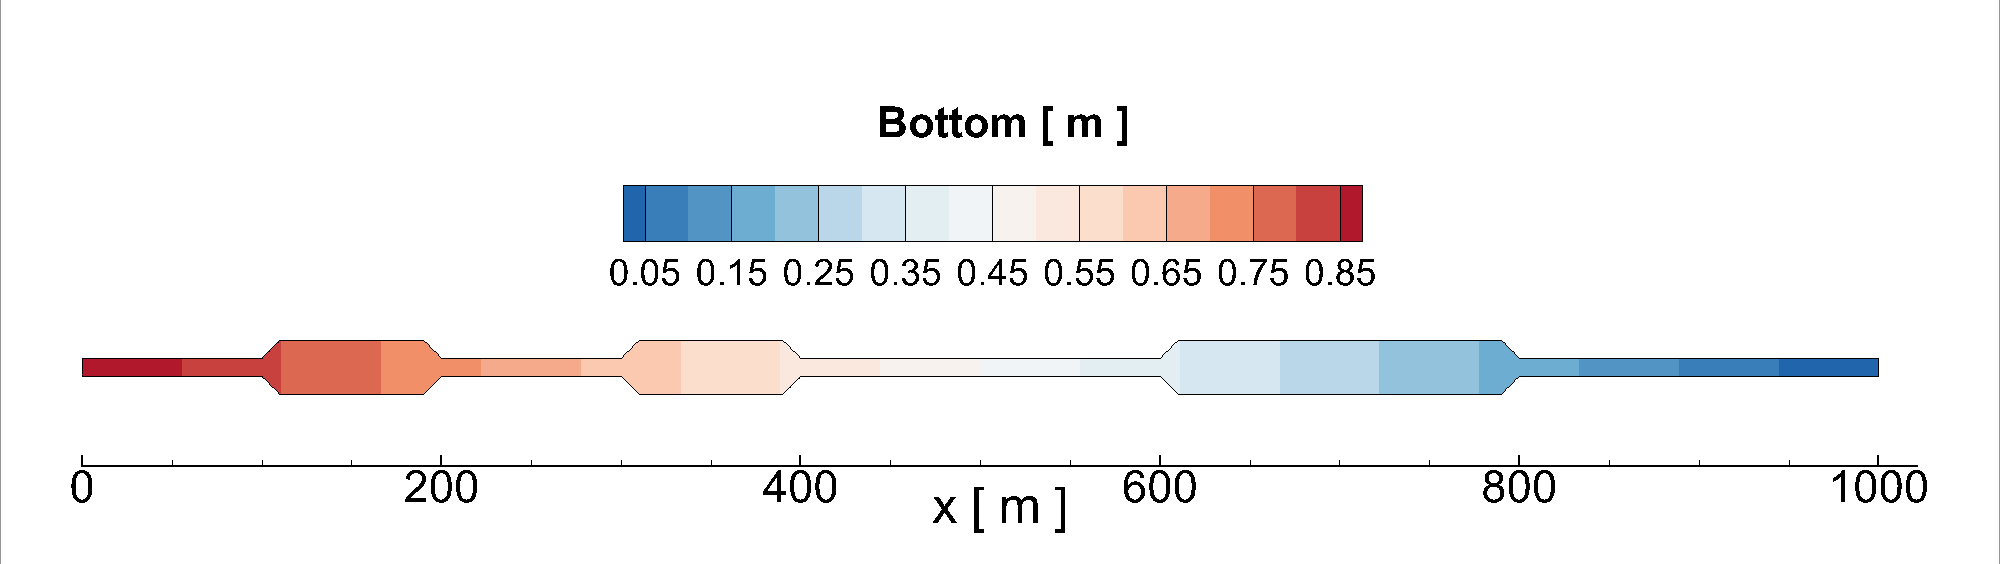
\includegraphics[scale=0.175]{img/ini_bottom.png}
 \caption{Geometry of the test flume with three wide sections}\label{E1iniBot}
\end{figure}



\newpage
%****************************************************
% - Initial and boundary conditions:
%     This part details both initial and boundary conditions used to simulate the case
\section{Initial and Boundary Conditions}
%
Steady state boundary conditions:\\
  \hspace*{3mm} - Discharge at the inlet = 20\,m$^3$/s\\
  \hspace*{3mm} - Water depth at outlet = 1\,m\\
  \hspace*{3mm} - Sedimentological equilibrium at the inlet (bottom level is constant,\\
  \hspace*{5.3mm} bedload transport will be calculated)\\
\\
Initial conditions hydraulic:\\
  \hspace*{3mm} - Fully developed flow from a previous simulation is used as hydraulic initial conditions.\\
\\
Initial conditions sedimentological:\\
  \hspace*{3mm} - The grain composition (fig.\,\ref{E1iniDm}) in the left part of the fulme consists completely of the\\
  \hspace*{5.3mm} grain class 1 (d\,=\,0.1\,mm). The right part consists completely of the grain class 3 (d\,=\,2.0\,mm).\\
  \hspace*{5.3mm} Grain class 2 is not present. These are preprocessing settings which are set in the\\
  \hspace*{5.3mm} \textsc{Previous Sedimentological Computation File}.\\
\\
\\
\\
%\newpage
\begin{figure} [!h]
\centering
 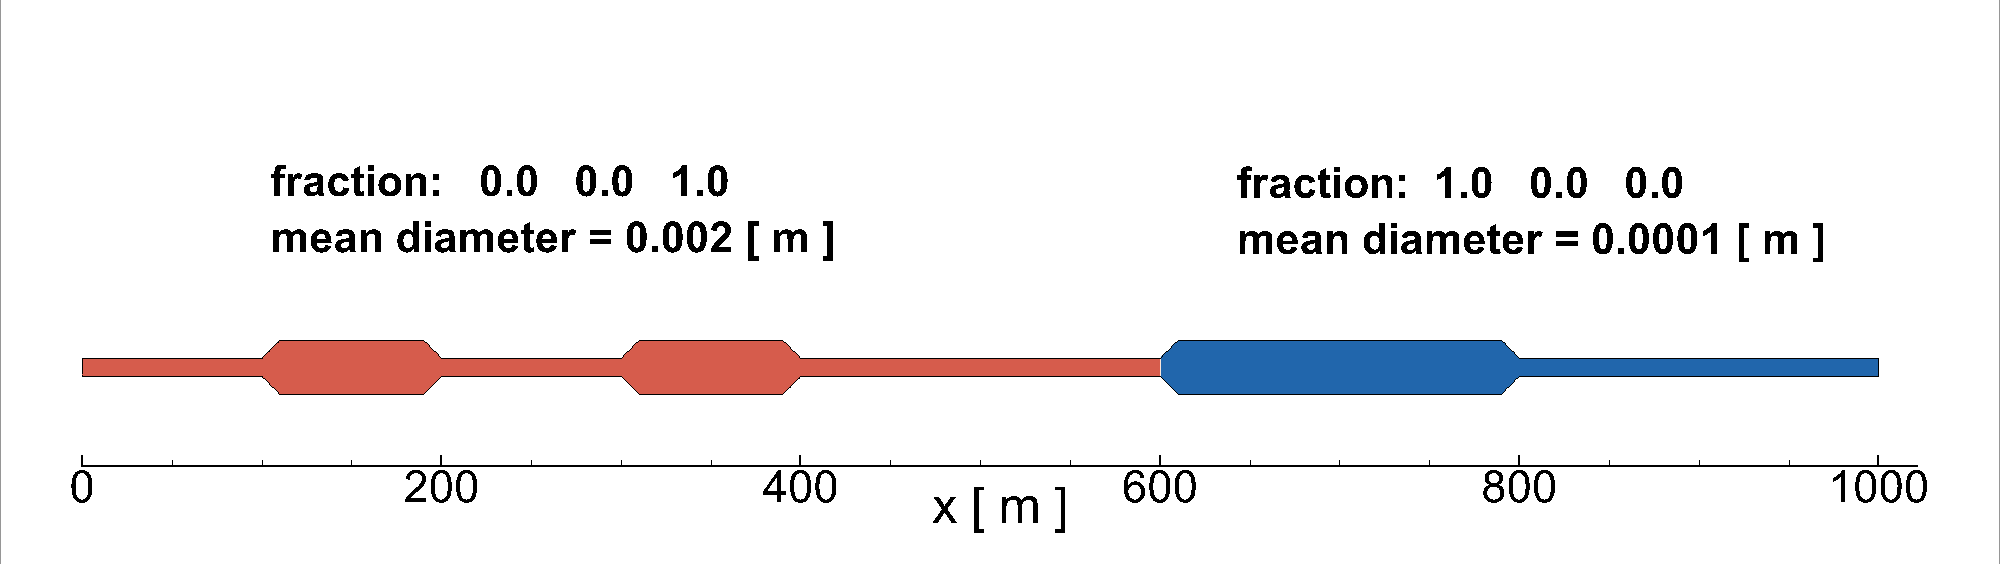
\includegraphics[scale=0.175]{img/ini_grainsize.png}
 \caption{Initial mean diameter in the active layer due to the distribution of the grain classes }\label{E1iniDm}
\end{figure}



\newpage
%****************************************************
\section{Results} \label{sec:E1Result}
%****************************************************
%
Information about when the Action was active and what was going on,
was printed (lines with \texttt{"\textbf{?>}"} at the beginning) into the telemac listing file.\\
%To find some information about when the Action was active and what was going on,
%search in the telemac listing file for lines with \texttt{"\textbf{?>}"} at the beginning. \\
\\
\label{txt:E1List}
Excerpt from the telemac listing with information about the Action status:\\
\\~\hspace*{3mm} \texttt{\small{~?>~:}}
\\~\hspace*{3mm}~\texttt{\small{~?>~info:========================================================+}}
\\~\hspace*{3mm}~\texttt{\small{~?>~info:~~~~~~~~~~~~~~~~~~~~~~~~~~~~~~~~~~~~~~~~~~~~~~~~~~~~~~~~|}}
\\~\hspace*{3mm}~\texttt{\small{~?>~info:~~~~~~~~~~~~NESTOR~~~~~~~~~~~~~~~~~~~~~~~~~~~~~~~~~~~~~~|}}
\\~\hspace*{3mm}~\texttt{\small{~?>~~~~~~~~~~~~~~~~~~~~~~~~~~~~~~~~~~~~~~~~~~~~~~~~~~~~~~~~~~~~~~~}}
\\~\hspace*{3mm}~\texttt{\small{~?>~~~~~~~~~~action~number~~~~:~~~1~~~~~~~~~~~~~~~~~~~~~~~~~~~~~~~}}
\\~\hspace*{3mm}~\texttt{\small{~?>~~~~~~~~~~~~~~~~~~~~~~~~~~~~~~~~~~~~~~~~~~~~~~~~~~~~~~~~~~~~~~~}}
\\~\hspace*{3mm}~\texttt{\small{~?>~~~~~~~~~~start~action~~~~~:~Dig\_by\_time~~~~~~~~~~~~~~~~~~~~~~~}}
\\~\hspace*{3mm}~\texttt{\small{~?>~~nominal~start~time~~[s]~~:~~~~50.000000000000000~~~~~~~~~~~~~}}
\\~\hspace*{3mm}~\texttt{\small{~?>~~~~~~~~~~start~time~~[s]~~:~~~~50.000000000000000~~~~~~~~~~~~~}}
\\~\hspace*{3mm}~\texttt{\small{~?>~~~~~~~~~~~~~~~~~~~~~~~~~~~~~~~~~~~~~~~~~~~~~~~~~~~~~~~~~~~~~~~}}
\\~\hspace*{3mm}~\texttt{\small{~?>~~~~~~~~~~FieldDig~~~~~~~~~:~201\_Abschnitt\_1\_2\_1000m**2~~~~~~~~}}
\\~\hspace*{3mm}~\texttt{\small{~?>~~~~~dz~per~time~step~[m]~~:~~~1.00000000000000002E-003~~~~~~~~}}
\\~\hspace*{3mm}~\texttt{\small{~?>~~~~~~~~~~~~~~~~~~~~~~~~~~~~~~~~~~~~~~~~~~~~~~~~~~~~~~~~~~~~~~~}}
\\~\hspace*{3mm}~\texttt{\small{~?>~~~~~~~~~~FieldDump~~~~~~~~:~202\_Abschnitt\_6\_7\_1000m**2~~~~~~~~}}
\\~\hspace*{3mm}~\texttt{\small{~?>~~~~~dz~per~time~step~[m]~~:~~~5.00000000000000010E-004~~~~~~~~}}
\\~\hspace*{3mm}~\texttt{\small{~?>~~~~~~~~~~~~~~~~~~~~~~~~~~~~~~~~~~~~~~~~~~~~~~~~~~~~~~~~~~~~~~~}}
\\~\hspace*{3mm}~\texttt{\small{~?>~info:~~~~~~~~~~~~~~~~~~~~~~~~~~~~~~~~~~~~~~~~~~~~~~~~~~~~~~~~|}}
\\~\hspace*{3mm}~\texttt{\small{~?>~info:========================================================+}}
\\~\hspace*{3mm} \texttt{\small{~?>~:}}
\\
\newpage
Figure~\ref{E1result50} shows the bed evolution after 50\,s (start of dredging and dumping),
after 100\,s (end of dredging) and after 250\,s (final simulation state and end of dumping process).

\begin{figure} [!h]
 \centering
 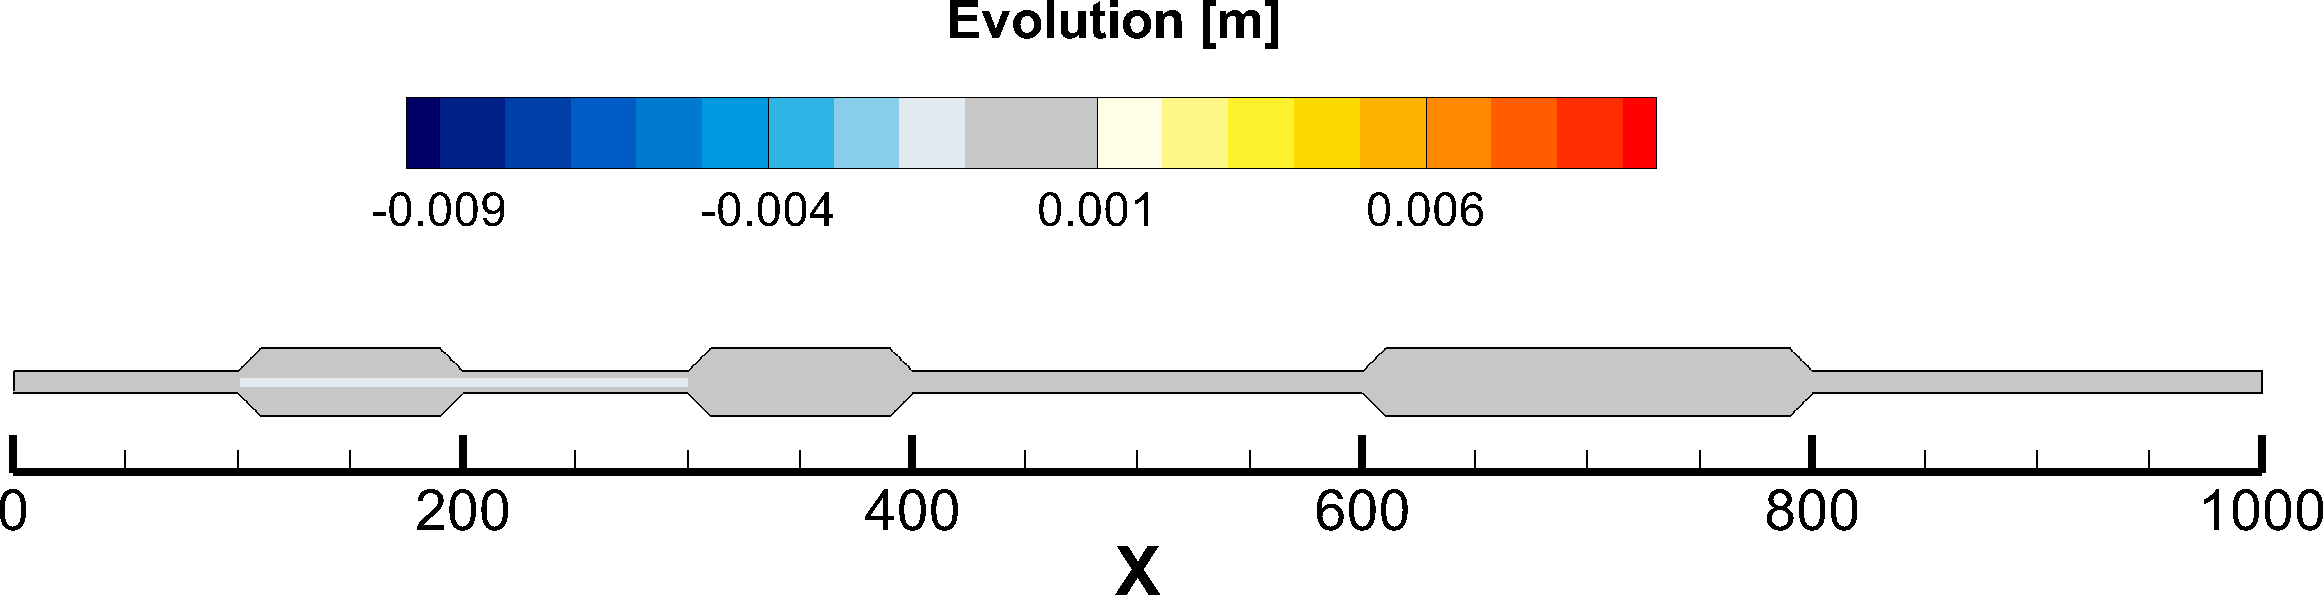
\includegraphics[scale=0.15]{img/result50.png}
 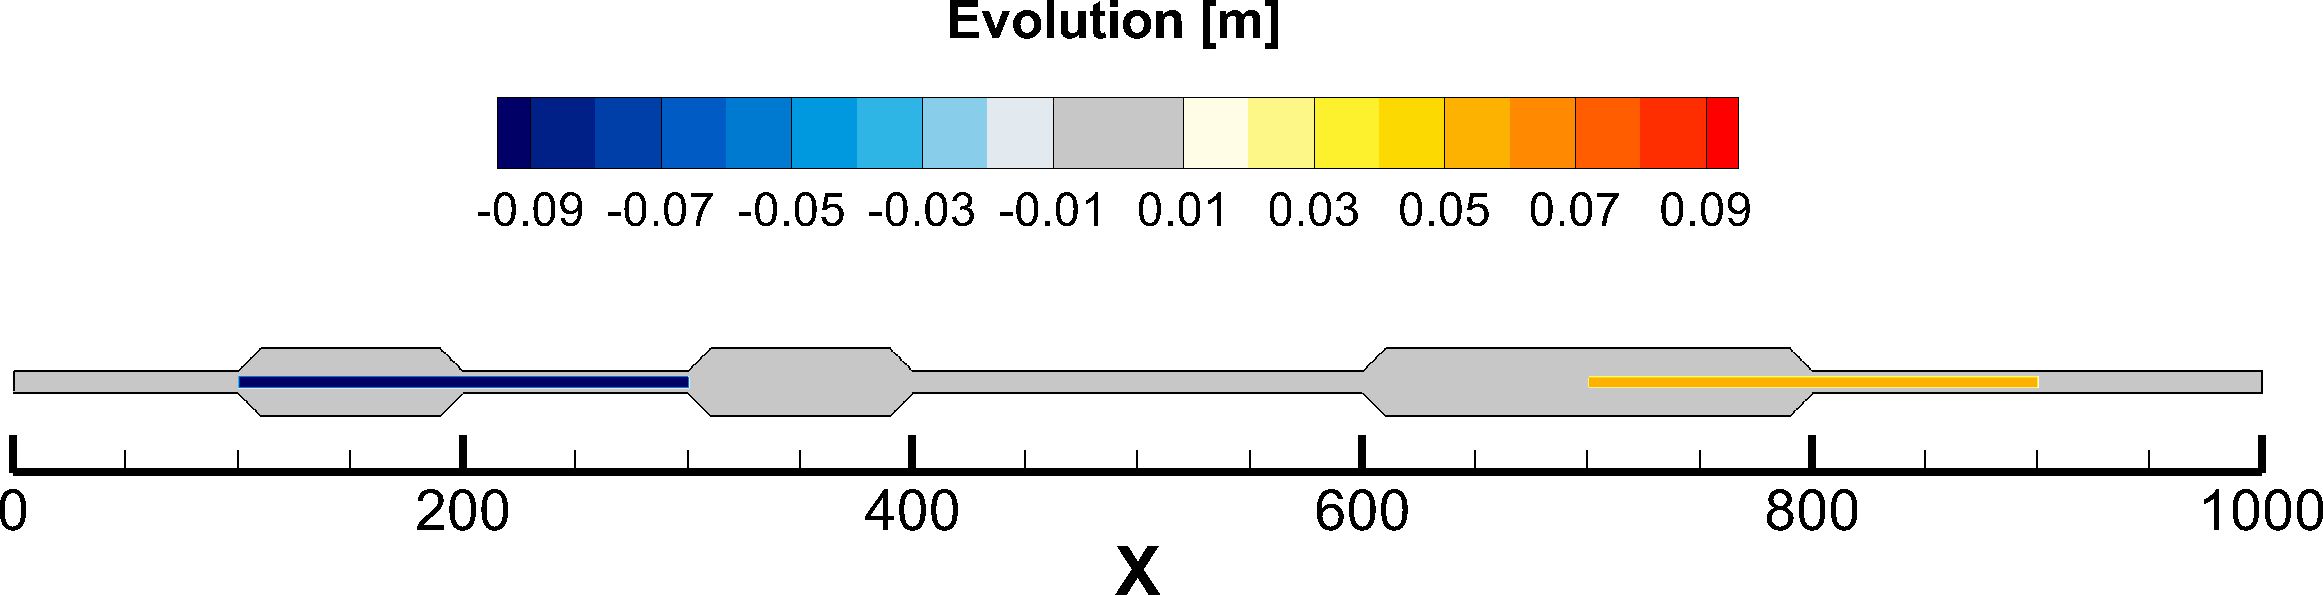
\includegraphics[scale=0.15]{img/result150.png}
 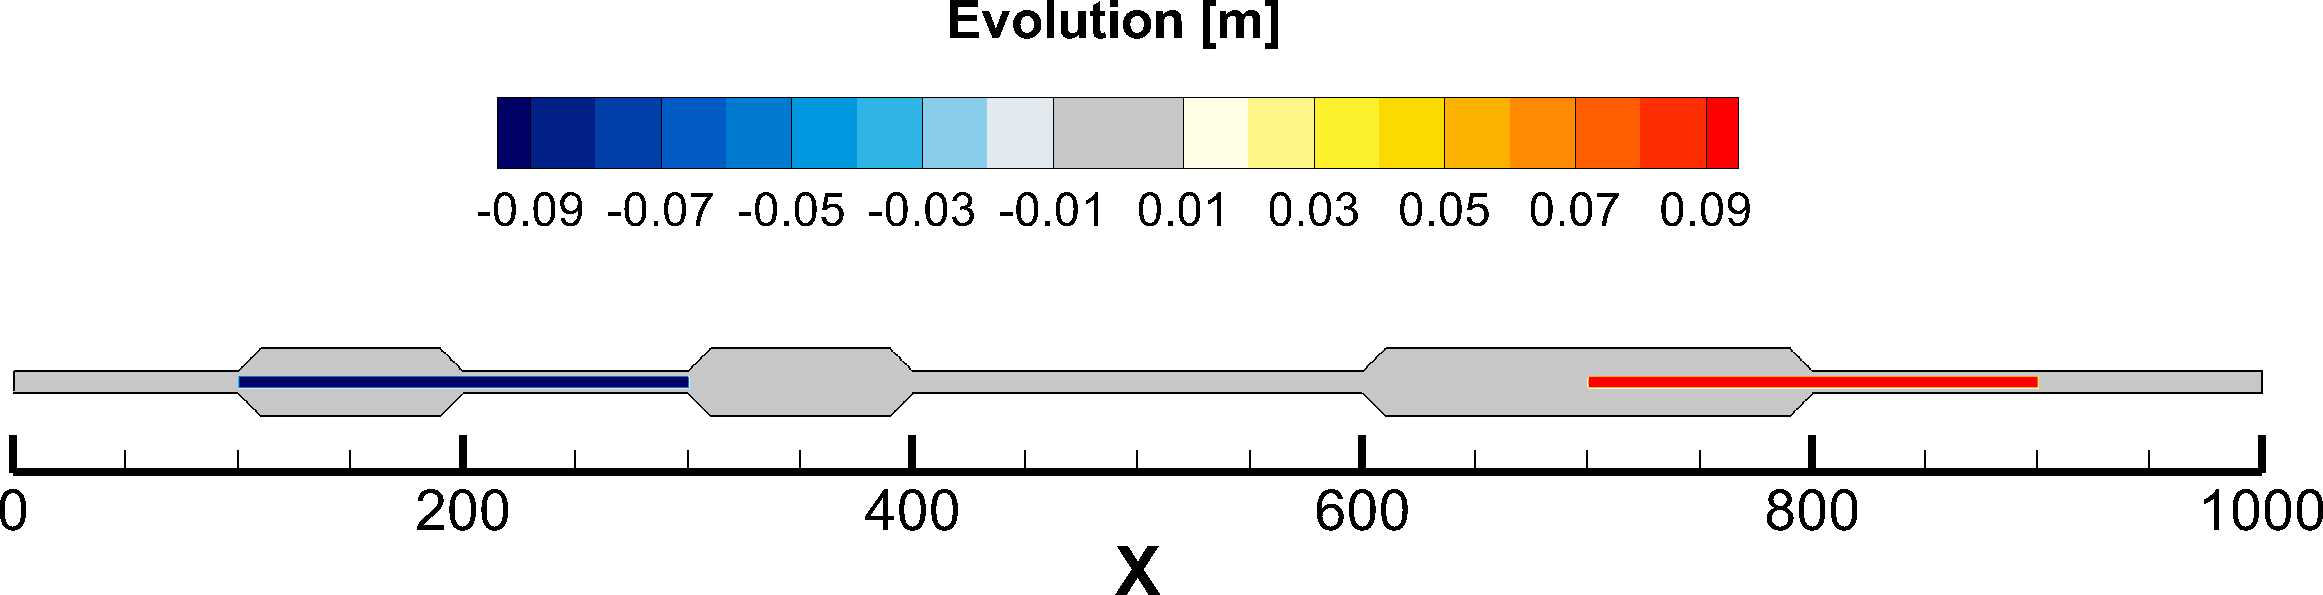
\includegraphics[scale=0.15]{img/result250.png}
 \caption{Simulated evolution after 50, 100 and 250\,s.}\label{E1result50}
\end{figure}
\textcolor{white}{force a empty line by white lettering} \\    %----- white line-----
\\
\\
\\
\\
\begin{figure} [!h]
 \centering
 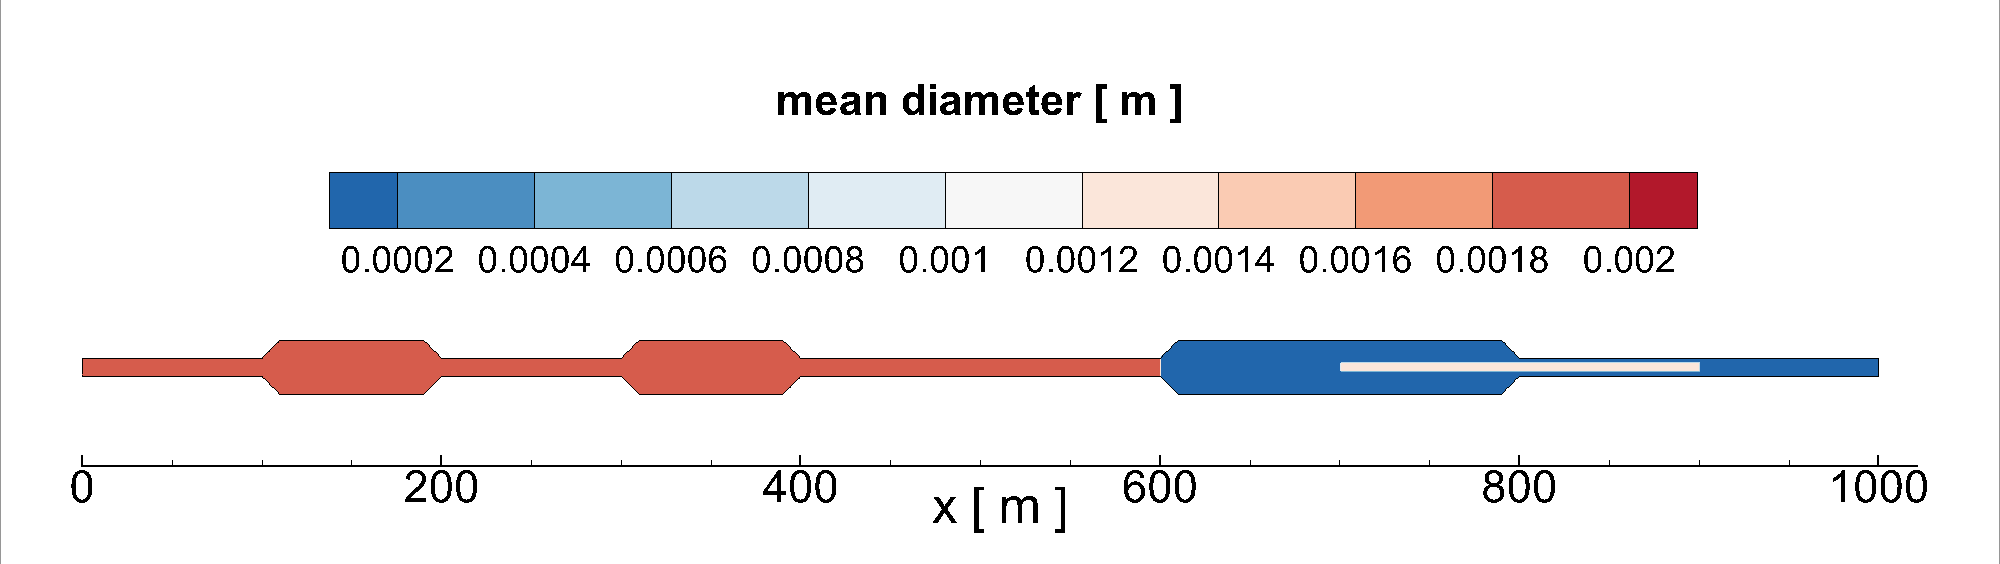
\includegraphics[scale=0.175]{img/final_grainsize.png}
 \caption{Final mean diameter in the active layer due to the distribution of the grain classes }\label{E1endDm}
\end{figure}
